\section{Experiment} \label{sec:simulation}
In this section, we compare the quality of the isometry of
conventional RPs, TRP, and TRP(5), for
Gaussian, Sparse \cite{achlioptas2003database},
and Very Sparse random maps \cite{li2006very} on both synthetic data and MNIST data.
We also use TRP and TRP(5) to compute pairwise cosine similarity
(Table \ref{tbl:mnist_inner_prod} and Appendix \ref{appendix:more_result})
and to sketch matrices and tensors
(Appendix \ref{appendix:sketching}),
although the theory still remains open.
% irrelevant, since we don't show timing
% We implemented the algorithm in Python and ran all experiments on a server with
% 128 Intel\textsuperscript{\textregistered} Xeon\textsuperscript{\textregistered} E7-4850
% v4 2.10GHz CPU cores and 1056GB memory.

Our first experiment evaluates the quality of the isometry for maps $\mathbb{R}^d \to \mathbb{R}^k$.
We generate $n=10$ independent vectors $\mathbf{x}_1, \dots, \mathbf{x}_n$ of sizes
$d = 2500, 10000, 40000$ from $\mathcal{N}(\mathbf{0},\mathbf{I})$.
We consider the following three RPs:
1. Gaussian RP; 2. Sparse RP \cite{achlioptas2003database}; 3. Very Sparse RP \cite{li2006very}.
For each, we compare the performance of RP, TRP, and TRP(5) with order 2 and $d_1=d_2$.
We evaluate the methods by repeatedly generating a RP and computing the reduced vector,
and plot the ratio of the pairwise distance
$\frac{1}{n(n-1)}\sum_{n \geq i\neq j \geq 1}\frac{\|\mathbf{A}\mathbf{x}_i - \mathbf{A}\mathbf{x}_j\|_2}{\|\mathbf{x}_i - \mathbf{x}_j\|_2}$
and the average standard deviation for different $k$
averaged over 100 replications.
In the MNIST example, we choose the first $n = 50$ vectors of size $d = 784$, normalize them,
and perform the same experiment.
Figure \ref{fig:main} shows results on simulated ($d = 2500$) and MNIST data
for the Gaussian and Very Sparse RP.
See \ref{appendix:more_result} for additional experiments.

These experiments show that to preserve pairwise distance and cosine similarity,
TRP performs nearly as well as RP for all three types of maps.
With only five replicates, TRP(5) reduces the variance significantly in real data while not much in the simulation setting.
The difference in accuracy between methods diminishes as $k$ increases.
When $d = d_1d_2 = 40000$, the storage for TRP(5) is still $\frac{1}{20}$ of the Gaussian RP.
The variance reduction is effective especially in sparse and very sparse setting.
% Furthermore, despite current lack of rigorous guarantee, the structured random map with variance reduction works very effective for sketching even when $d = 1000000$.
%For further investigation of the effect of our structured random map on matrix sketching, please refer to Appendix \ref{appendix:sketching}.
\begin{figure}[H]
	\centering
	\begin{subfigure}{0.24\textwidth}
		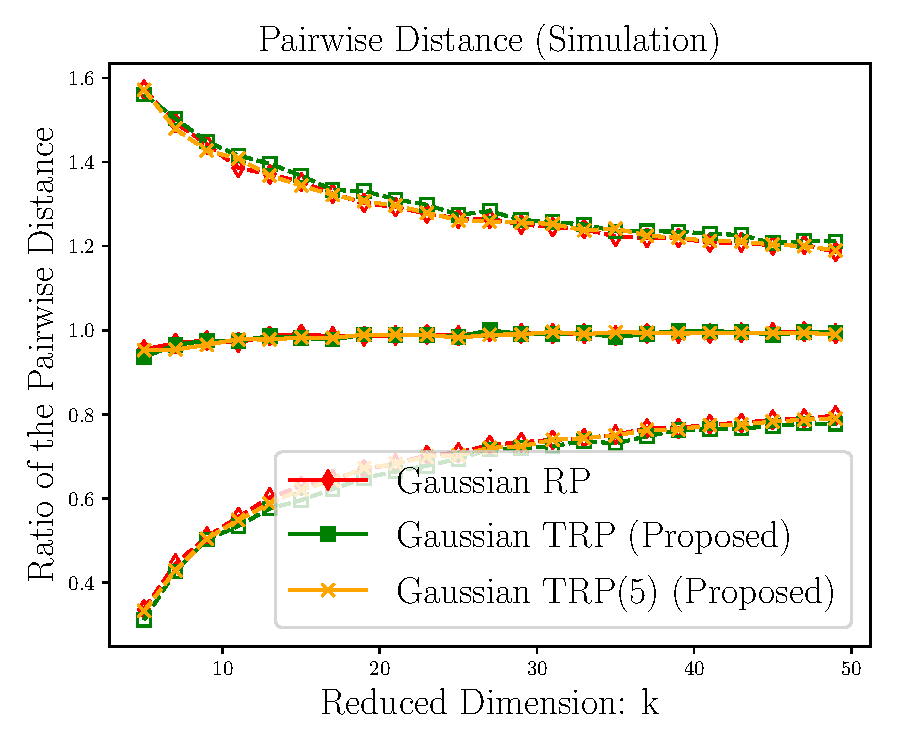
\includegraphics[scale = 0.22]{figure/dist_g_d2500.pdf}
	\end{subfigure}
	\begin{subfigure}{0.24\textwidth}
		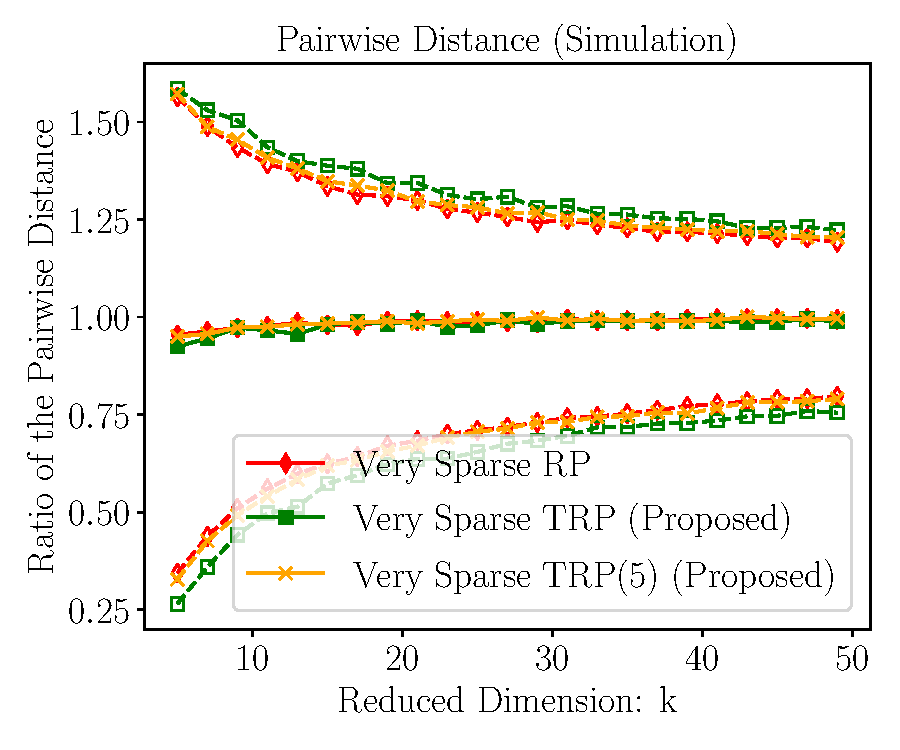
\includegraphics[scale = 0.22]{figure/dist_sp1_d2500.pdf}
	\end{subfigure}
	\begin{subfigure}{0.24\textwidth}
		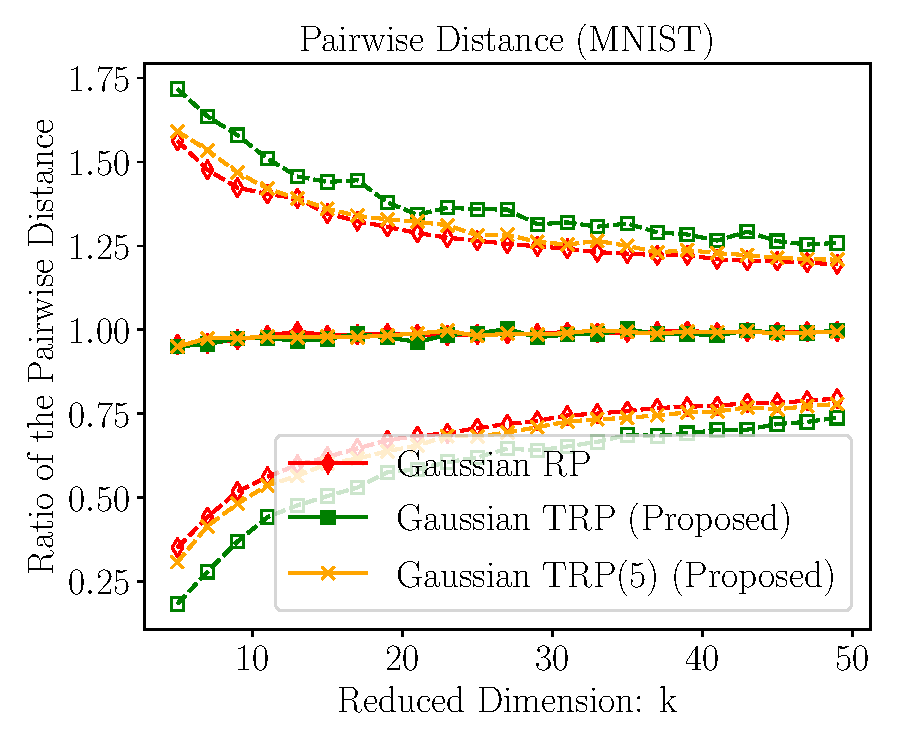
\includegraphics[scale = 0.22]{figure/dist_g_mnist.pdf}
	\end{subfigure}
	\begin{subfigure}{0.24\textwidth}
		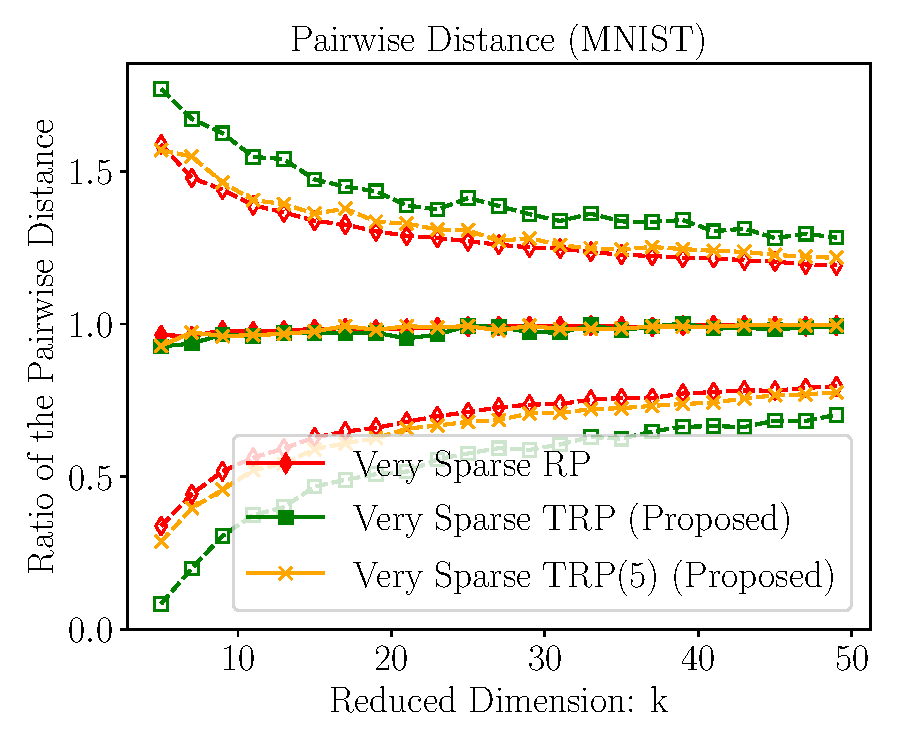
\includegraphics[scale = 0.22]{figure/dist_sp1_mnist.pdf}
	\end{subfigure}\\
	\caption{Isometry quality for simulated and MNIST data.
		The left two plots show results for Gaussian and Very Sparse RP, TRP, TRP(5)
		respectively applied to $n = 20$ standard normal data vectors in $\mathbb{R}^{2500}$.
		The right two plots show the same for 50 MNIST image vectors in $\mathbb{R}^{784}$.
		The dashed line shows the error two standard deviations from the average ratio.}
	\label{fig:main}
\end{figure}

\begin{table}[H]
	\centering
	\begin{tabular}{l|l|l|l}
		& Gaussian        & Sparse          & Very Sparse     \\ \hline
		RP & 0.1198 (0.0147) & 0.1198 (0.0150) & 0.1189 (0.0108) \\ \hline
		TRP    & 0.1540 (0.0290) & 0.1609 (0.0335) & 0.1662 (0.0307) \\ \hline
		TRP(5) & 0.1262 (0.0166) & 0.1264 (0.0194) & 0.1276 (0.0164)
	\end{tabular}
	\caption{RMSE for the estimate of the pairwise inner product of the MNIST data, where standard error is in the parentheses.} \label{tbl:mnist_inner_prod}
\end{table}